\newpage
\section{Проектирование}
\label{sec:Definition}
 
\subsection{Требования к системе}
В ходе проектирования приложения были определены следующие функциональные и нефункциональные требования.

\textbf{Функциональные требования.}

Функциональные требования определяют действия, которые должна выполнять программа.
\begin{enumerateparen}
    \item В программе должна быть возможность разметить текст песни.
    \item Программа должна отделять припевы от куплетов.
    \item Программа должна визуализировать результаты работы алгоритма, показывать какие части текста были классифицированы правильно и неправильно.
\end{enumerateparen}

\textbf{Нефункциональные требования.}

Нефункциональные действия определяют свойства программы (удобство использования, безопасность и т.д.). 
\begin{enumerateparen}
    \item Приложение должно иметь понятный для использования пользовательский интерфейс.
    \item Реализация программы осуществляется с использованием языка Python.
    \item Пользовательский интерфейс должен быть реализован с использованием библиотеки Tkinter.
\end{enumerateparen}


\vspace{2em}
\subsection{Варианты использования системы}
Для проектирования приложения был использован язык графического
описания для объектного моделирования UML. Была построена модель взаимодействия пользователя с приложением в виде диаграммы вариантов использования (рисунок~\ref{fig:Варианты использования}). 
В ходе анализа разрабатываемого приложения были выявлены основные варианты использования.
\begin{figure}[h]
    \centering
    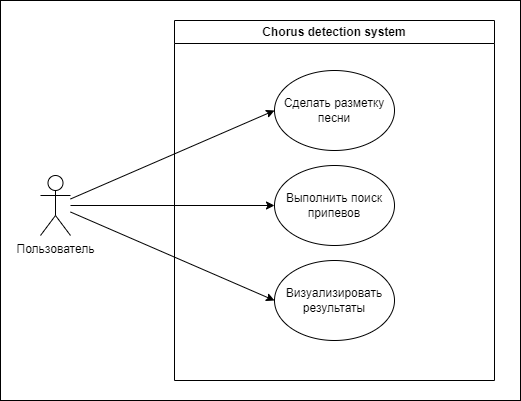
\includegraphics[width=1\linewidth]{pictures/Варианты использования.png}
    \caption{Варианты использования приложения}
    \label{fig:Варианты использования}
\end{figure}

\begin{enumerateparen}
    \item Вариант <<Сделать разметку песни>>. Пользователь может воспользоваться утилитой разметки, чтобы самостоятельно отделить припевы от остальных частей песни, а так же указать информацию о длине припева в символах, количестве различных частей песни.
    \item Вариант <<Выполнить поиск припевов>>. Пользователь может запустить процесс, выделяющий припевы из текста песни. Он может указать параметры, необходимые для работы алгоритма, такие как длина припева, количество отрезков песни, являющихся припевами.
    \item Вариант <<Визуализировать результаты>>. Пользователь может оценить качество работы алгоритма, открыв дополнительное окно с визуализацией разметки. 
\end{enumerateparen}

\vspace{2em}
\subsection{Архитектура приложения}
В данном разделе рассматривается спроектированная архитектура
приложения в виде диаграммы компонентов, которая показывает разбиение
системы на структурные компоненты. Спроектированная архитектура приложения представлена на рисунке~\ref{fig:Структура}  в виде диаграммы компонентов.

\begin{figure}[h]
    \centering
    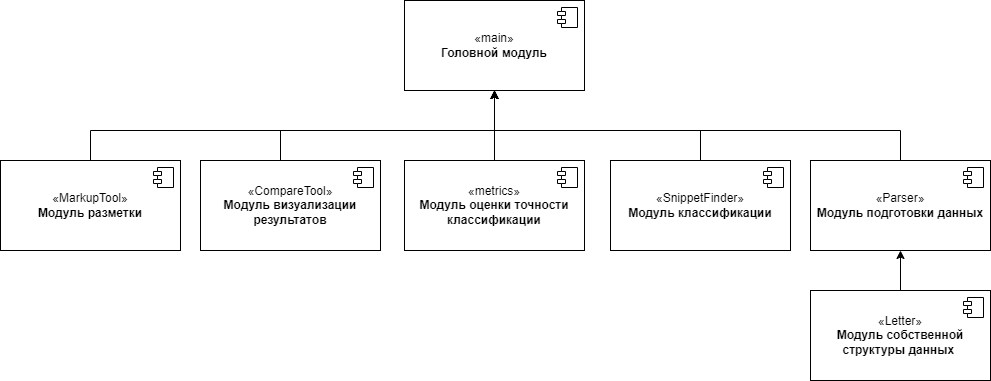
\includegraphics[width=1\linewidth]{pictures/Структура.png}
    \caption{Архитектура приложения}
    \label{fig:Структура}
\end{figure}

Компонент \textit{головной модуль} выполняет отображение окон приложения, с которыми может взаимодействовать пользователь, и осуществляет запуск подчиненных модулей приложения.

\textit{Модуль разметки} является утилитой, позволяющей подготовить текст песни к использованию в приложении. Данный этап предполагает загрузку текста песни в формате txt, разделение пользователем песни на сегменты, указание метаданных, и выгрузку размеченной песни в формате xml.

\textit{Модуль визуализации} позволяет сравнить оригинальную разметку песни с разметкой, полученной в результате работы алгоритма. Для удобства использования неправильно классифицированные фрагменты текста выделяются красным цветом.

\textit{Модуль оценки точности} представляет собой набор алгоритмов, позволяющих оценить корректность полученной разметки. В данном модуле используются такие метрики как accuracy, precision, recall и F-score.  

\textit{Структура данных Letter} представляет символ текста песни как отдельный объект, который будет рассматриваться в ходе работы алгоритма. Данная структура, помимо самого символа, содержит acsii-код данного символа, информацию о том в какой части песни он находится, куда его определил алгоритм классификации, а так же, является ли эта классификация ошибочной. 

\textit{Модуль подготовки данных} используется для загрузки текста песни в приложение. Данный компонент отвечает за работу с внешними файлами и может работать как с форматом txt, так и с форматом xml. Кроме того, данный модуль преобразует текст песни в массив вышеописанных структур, который затем используется в работе алгоритма.

\textit{Модуль классификации} представляет собой основной алгоритм программы. Он по заданным параметрам ищет в массиве символов наиболее повторяющуюся подпоследовательность и классифицирует ее как припев. Так, результатом работы является размеченный массив символов, который передается в модуль визуализации и модуль оценки точности для просмотра результата работы.

\vspace{2em}
\subsection{Графический интерфейс}
В данном разделе будут представлены спроектированные макеты
пользовательского интерфейса приложения. Данные макеты являются примерным представлением итогового продукта и содержат в себе основные
необходимые функции.

Окно разметки содержит текстовое поле, в котором можно посмотреть текущую разметку, поле для ввода номера, поле для выбора раздела песни, поле для выбора метаданных. А так же две кнопки, при нажатии на которые, автоматически расставляются xml теги в зависимости от выбранных параметров. На рисунке~\ref{fig:Разметка} представлен макет окна разметки.

\begin{figure}
    \centering
    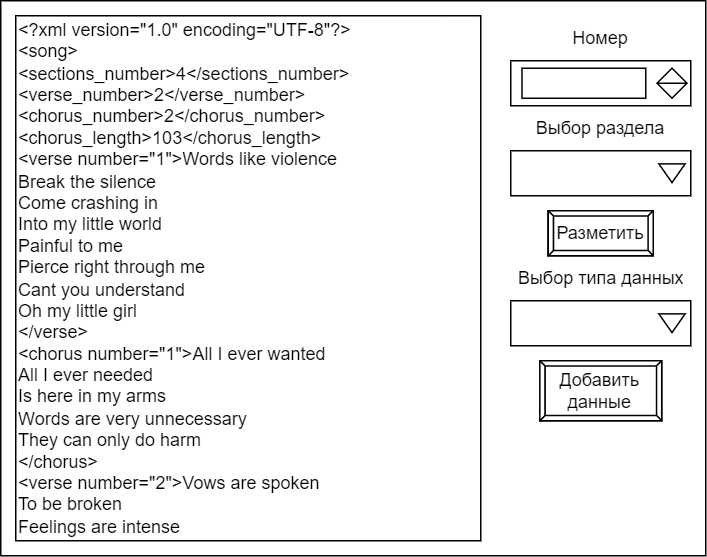
\includegraphics[width=1\linewidth]{pictures/Разметка.png}
    \caption{Макет окна разметки}
    \label{fig:Разметка}
\end{figure}

Окно визуализации результатов представляет собой три текстовых поля. В первом поле находится текст песни, в том виде, в котором он поступил на вход программы. Во втором поле находится истинная разметка песни. Припевы и куплеты в данном случае выбелены различными цветами, припевы — зеленым, куплеты — синем. В третьем поле находится текст песни, размеченный алгоритмом. Части данного цвета, также выделяются цветами. Если символ классифицирован корректно, он отмечается цветом своего раздела, синий или зеленый. В случае если символ классифицирован неверно, он отмечается красным цветом. На рисунке~\ref{fig:Визуализация} представлен макет окна визуализации.

\begin{figure}
    \centering
    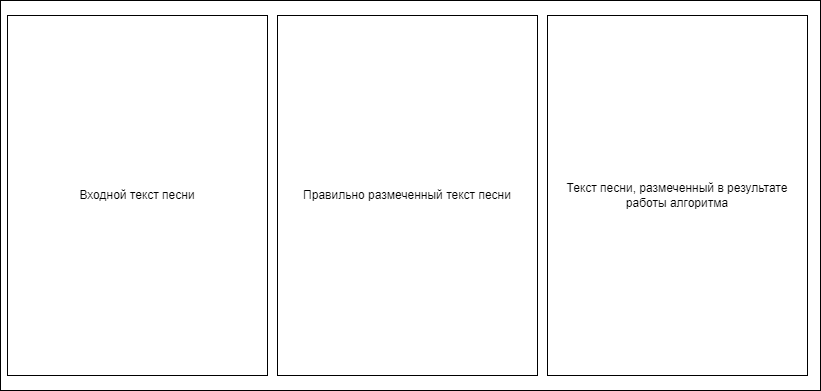
\includegraphics[width=1\linewidth]{pictures/Визуализация.png}
    \caption{Макет окна визуализации}
    \label{fig:Визуализация}
\end{figure}